% Generated by Sphinx.
\def\sphinxdocclass{report}
\documentclass[letterpaper,10pt,oneside]{sphinxmanual}
\usepackage[utf8]{inputenc}
\DeclareUnicodeCharacter{00A0}{\nobreakspace}
\usepackage[T1]{fontenc}
\usepackage[english]{babel}
\usepackage{times}
\usepackage[Bjarne]{fncychap}
\usepackage{longtable}
\usepackage{sphinx}
\usepackage{multirow}


\title{PyCelegans Documentation}
\date{May 11, 2012}
\release{0}
\author{Nicholas P. Labello}
\newcommand{\sphinxlogo}{}
\renewcommand{\releasename}{Release}
\makeindex

\makeatletter
\def\PYG@reset{\let\PYG@it=\relax \let\PYG@bf=\relax%
    \let\PYG@ul=\relax \let\PYG@tc=\relax%
    \let\PYG@bc=\relax \let\PYG@ff=\relax}
\def\PYG@tok#1{\csname PYG@tok@#1\endcsname}
\def\PYG@toks#1+{\ifx\relax#1\empty\else%
    \PYG@tok{#1}\expandafter\PYG@toks\fi}
\def\PYG@do#1{\PYG@bc{\PYG@tc{\PYG@ul{%
    \PYG@it{\PYG@bf{\PYG@ff{#1}}}}}}}
\def\PYG#1#2{\PYG@reset\PYG@toks#1+\relax+\PYG@do{#2}}

\def\PYG@tok@gd{\def\PYG@tc##1{\textcolor[rgb]{0.63,0.00,0.00}{##1}}}
\def\PYG@tok@gu{\let\PYG@bf=\textbf\def\PYG@tc##1{\textcolor[rgb]{0.50,0.00,0.50}{##1}}}
\def\PYG@tok@gt{\def\PYG@tc##1{\textcolor[rgb]{0.00,0.25,0.82}{##1}}}
\def\PYG@tok@gs{\let\PYG@bf=\textbf}
\def\PYG@tok@gr{\def\PYG@tc##1{\textcolor[rgb]{1.00,0.00,0.00}{##1}}}
\def\PYG@tok@cm{\let\PYG@it=\textit\def\PYG@tc##1{\textcolor[rgb]{0.25,0.50,0.56}{##1}}}
\def\PYG@tok@vg{\def\PYG@tc##1{\textcolor[rgb]{0.73,0.38,0.84}{##1}}}
\def\PYG@tok@m{\def\PYG@tc##1{\textcolor[rgb]{0.13,0.50,0.31}{##1}}}
\def\PYG@tok@mh{\def\PYG@tc##1{\textcolor[rgb]{0.13,0.50,0.31}{##1}}}
\def\PYG@tok@cs{\def\PYG@tc##1{\textcolor[rgb]{0.25,0.50,0.56}{##1}}\def\PYG@bc##1{\colorbox[rgb]{1.00,0.94,0.94}{##1}}}
\def\PYG@tok@ge{\let\PYG@it=\textit}
\def\PYG@tok@vc{\def\PYG@tc##1{\textcolor[rgb]{0.73,0.38,0.84}{##1}}}
\def\PYG@tok@il{\def\PYG@tc##1{\textcolor[rgb]{0.13,0.50,0.31}{##1}}}
\def\PYG@tok@go{\def\PYG@tc##1{\textcolor[rgb]{0.19,0.19,0.19}{##1}}}
\def\PYG@tok@cp{\def\PYG@tc##1{\textcolor[rgb]{0.00,0.44,0.13}{##1}}}
\def\PYG@tok@gi{\def\PYG@tc##1{\textcolor[rgb]{0.00,0.63,0.00}{##1}}}
\def\PYG@tok@gh{\let\PYG@bf=\textbf\def\PYG@tc##1{\textcolor[rgb]{0.00,0.00,0.50}{##1}}}
\def\PYG@tok@ni{\let\PYG@bf=\textbf\def\PYG@tc##1{\textcolor[rgb]{0.84,0.33,0.22}{##1}}}
\def\PYG@tok@nl{\let\PYG@bf=\textbf\def\PYG@tc##1{\textcolor[rgb]{0.00,0.13,0.44}{##1}}}
\def\PYG@tok@nn{\let\PYG@bf=\textbf\def\PYG@tc##1{\textcolor[rgb]{0.05,0.52,0.71}{##1}}}
\def\PYG@tok@no{\def\PYG@tc##1{\textcolor[rgb]{0.38,0.68,0.84}{##1}}}
\def\PYG@tok@na{\def\PYG@tc##1{\textcolor[rgb]{0.25,0.44,0.63}{##1}}}
\def\PYG@tok@nb{\def\PYG@tc##1{\textcolor[rgb]{0.00,0.44,0.13}{##1}}}
\def\PYG@tok@nc{\let\PYG@bf=\textbf\def\PYG@tc##1{\textcolor[rgb]{0.05,0.52,0.71}{##1}}}
\def\PYG@tok@nd{\let\PYG@bf=\textbf\def\PYG@tc##1{\textcolor[rgb]{0.33,0.33,0.33}{##1}}}
\def\PYG@tok@ne{\def\PYG@tc##1{\textcolor[rgb]{0.00,0.44,0.13}{##1}}}
\def\PYG@tok@nf{\def\PYG@tc##1{\textcolor[rgb]{0.02,0.16,0.49}{##1}}}
\def\PYG@tok@si{\let\PYG@it=\textit\def\PYG@tc##1{\textcolor[rgb]{0.44,0.63,0.82}{##1}}}
\def\PYG@tok@s2{\def\PYG@tc##1{\textcolor[rgb]{0.25,0.44,0.63}{##1}}}
\def\PYG@tok@vi{\def\PYG@tc##1{\textcolor[rgb]{0.73,0.38,0.84}{##1}}}
\def\PYG@tok@nt{\let\PYG@bf=\textbf\def\PYG@tc##1{\textcolor[rgb]{0.02,0.16,0.45}{##1}}}
\def\PYG@tok@nv{\def\PYG@tc##1{\textcolor[rgb]{0.73,0.38,0.84}{##1}}}
\def\PYG@tok@s1{\def\PYG@tc##1{\textcolor[rgb]{0.25,0.44,0.63}{##1}}}
\def\PYG@tok@gp{\let\PYG@bf=\textbf\def\PYG@tc##1{\textcolor[rgb]{0.78,0.36,0.04}{##1}}}
\def\PYG@tok@sh{\def\PYG@tc##1{\textcolor[rgb]{0.25,0.44,0.63}{##1}}}
\def\PYG@tok@ow{\let\PYG@bf=\textbf\def\PYG@tc##1{\textcolor[rgb]{0.00,0.44,0.13}{##1}}}
\def\PYG@tok@sx{\def\PYG@tc##1{\textcolor[rgb]{0.78,0.36,0.04}{##1}}}
\def\PYG@tok@bp{\def\PYG@tc##1{\textcolor[rgb]{0.00,0.44,0.13}{##1}}}
\def\PYG@tok@c1{\let\PYG@it=\textit\def\PYG@tc##1{\textcolor[rgb]{0.25,0.50,0.56}{##1}}}
\def\PYG@tok@kc{\let\PYG@bf=\textbf\def\PYG@tc##1{\textcolor[rgb]{0.00,0.44,0.13}{##1}}}
\def\PYG@tok@c{\let\PYG@it=\textit\def\PYG@tc##1{\textcolor[rgb]{0.25,0.50,0.56}{##1}}}
\def\PYG@tok@mf{\def\PYG@tc##1{\textcolor[rgb]{0.13,0.50,0.31}{##1}}}
\def\PYG@tok@err{\def\PYG@bc##1{\fcolorbox[rgb]{1.00,0.00,0.00}{1,1,1}{##1}}}
\def\PYG@tok@kd{\let\PYG@bf=\textbf\def\PYG@tc##1{\textcolor[rgb]{0.00,0.44,0.13}{##1}}}
\def\PYG@tok@ss{\def\PYG@tc##1{\textcolor[rgb]{0.32,0.47,0.09}{##1}}}
\def\PYG@tok@sr{\def\PYG@tc##1{\textcolor[rgb]{0.14,0.33,0.53}{##1}}}
\def\PYG@tok@mo{\def\PYG@tc##1{\textcolor[rgb]{0.13,0.50,0.31}{##1}}}
\def\PYG@tok@mi{\def\PYG@tc##1{\textcolor[rgb]{0.13,0.50,0.31}{##1}}}
\def\PYG@tok@kn{\let\PYG@bf=\textbf\def\PYG@tc##1{\textcolor[rgb]{0.00,0.44,0.13}{##1}}}
\def\PYG@tok@o{\def\PYG@tc##1{\textcolor[rgb]{0.40,0.40,0.40}{##1}}}
\def\PYG@tok@kr{\let\PYG@bf=\textbf\def\PYG@tc##1{\textcolor[rgb]{0.00,0.44,0.13}{##1}}}
\def\PYG@tok@s{\def\PYG@tc##1{\textcolor[rgb]{0.25,0.44,0.63}{##1}}}
\def\PYG@tok@kp{\def\PYG@tc##1{\textcolor[rgb]{0.00,0.44,0.13}{##1}}}
\def\PYG@tok@w{\def\PYG@tc##1{\textcolor[rgb]{0.73,0.73,0.73}{##1}}}
\def\PYG@tok@kt{\def\PYG@tc##1{\textcolor[rgb]{0.56,0.13,0.00}{##1}}}
\def\PYG@tok@sc{\def\PYG@tc##1{\textcolor[rgb]{0.25,0.44,0.63}{##1}}}
\def\PYG@tok@sb{\def\PYG@tc##1{\textcolor[rgb]{0.25,0.44,0.63}{##1}}}
\def\PYG@tok@k{\let\PYG@bf=\textbf\def\PYG@tc##1{\textcolor[rgb]{0.00,0.44,0.13}{##1}}}
\def\PYG@tok@se{\let\PYG@bf=\textbf\def\PYG@tc##1{\textcolor[rgb]{0.25,0.44,0.63}{##1}}}
\def\PYG@tok@sd{\let\PYG@it=\textit\def\PYG@tc##1{\textcolor[rgb]{0.25,0.44,0.63}{##1}}}

\def\PYGZbs{\char`\\}
\def\PYGZus{\char`\_}
\def\PYGZob{\char`\{}
\def\PYGZcb{\char`\}}
\def\PYGZca{\char`\^}
\def\PYGZsh{\char`\#}
\def\PYGZpc{\char`\%}
\def\PYGZdl{\char`\$}
\def\PYGZti{\char`\~}
% for compatibility with earlier versions
\def\PYGZat{@}
\def\PYGZlb{[}
\def\PYGZrb{]}
\makeatother

\begin{document}

\maketitle
\tableofcontents
\phantomsection\label{index::doc}

\phantomsection\label{index:module-background}\index{background (module)}

\chapter{background}
\label{index:background}\label{index:welcome-to-pycelegans-s-documentation}
This executable builds a composite background image by taking the 
brightest pixel from a series of images.  By compositing multiple
images the worm, which blocks light and always darkens a pixel,
is effectively removed leaving a background which can be
subtracted from individual images.  Subtracting a background image
results in much cleaner segmentation and subsequent 
identification of worm properties (head, tail, sides, etc.).

usage: background.py {[}-h{]} {[}--imgdir IMGDIR{]} {[}--Nimg NIMG{]}
\begin{description}
\item[{optional arguments:}] \leavevmode\begin{optionlist}{3cm}
\item [-h, -{-}help]  
show this help message and exit
\item [-{-}imgdir IMGDIR]  
directory where input images are stored
\item [-{-}Nimg NIMG]  
Number of images to use to construct the background. The images
are spaced as far apart as possible.  For example, if 100 images are available
and Nimg=10, then image 1,11,21,31...91 would be used.
\item [-{-}windowsize WINDOWSIZE]  
Width of window used for background image generation.
This is the number of sequential frames that will use
the same background image. For example, if there are
10,000 frames, and --windowsize=1000, ten background
images will be generated. (default: 1)
\end{optionlist}

\end{description}

\scalebox{0.600000}{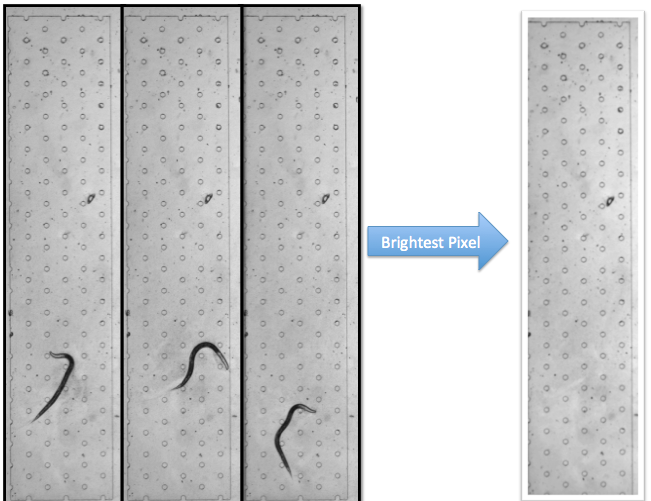
\includegraphics{brightest-pixel-composite.png}}
\phantomsection\label{index:module-creatediffimage}\index{creatediffimage (module)}

\chapter{creatediffimage}
\label{index:creatediffimage}
This stand alone executable builds a new image with the following
operation.
\begin{quote}

((background - image) \textgreater{} THRESH) * image
\end{quote}

\emph{background} will be approximately equally bright as \emph{image} on every
pixel that the worm does not occupy in \emph{image} (roughly +/- 10 based on 
0-255 range possible with 8 bit grayscale images).

Pixels that the worm occupies will be substantially darker (lower) in \emph{image} 
than background, by an intensity of 20 or more.  The image that is segmented 
and used for analysis is generated by the following steps.
\begin{enumerate}
\item {} \begin{description}
\item[{subtract \emph{image} from \emph{background}, result 8 bit array}] \leavevmode
tempimage = background - image

\end{description}

\item {} \begin{description}
\item[{generate binary array where \emph{tempimage} is greater than THRESH}] \leavevmode
temp2image = tempimage \textgreater{} THRESH

\end{description}

\item {} \begin{description}
\item[{multiply \emph{temp2image} by \emph{image}.  }] \leavevmode
finalimage = temp2image * image

\end{description}

\end{enumerate}

As a result, if THRESH is chosen well, \emph{finalimage} will contain only one major 
object, the worm.  Segmentation and analysis of \emph{finalimage} results in vastly
cleaner identification of worm head/tail/border than segmentation/analysis of
\begin{itemize}
\item {} 
Usage:  creatediffimage.py {[}background.jpg{]} {[}image.jpg{]} {[}THRESH{]}

\end{itemize}

\scalebox{0.800000}{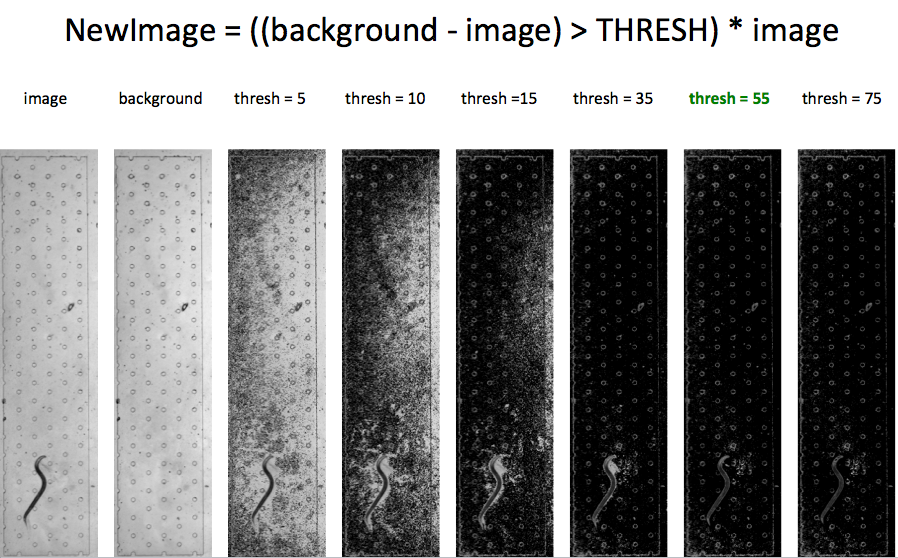
\includegraphics{diffimages.png}}
\phantomsection\label{index:module-preprocessajp}\index{preprocessajp (module)}

\chapter{preprocessajp}
\label{index:preprocessajp}
This executable splits AJP movies into individual jpeg images.  Given a root
directory preprocessajp will traverse down the file system recursively to find
all .ajp files.  Images are named with the movie prefix and a unique frame 
number.
\begin{description}
\item[{usage: preprocessajp.py {[}-h{]} {[}--np NPROCS{]} {[}--imgdir IMGDIR{]} --ajpdir AJPDIR}] \leavevmode
{[}--prefix PREFIX{]} {[}--nzerom NZEROM{]} {[}--nzeroa NZEROA{]}

\item[{Convert AJP movies to images. }] \leavevmode
Usage: preprocessajp.py {[}Directory of AJP Files{]}

\item[{optional arguments:}] \leavevmode\begin{optionlist}{3cm}
\item [-h, -{-}help]  
show this help message and exit
\item [-{-}np NPROCS]  
number of processors
\item [-{-}imgdir IMGDIR]  
directory where output images are stored
\item [-{-}ajpdir AJPDIR]  
directory where input AJP movies are found
\item [-{-}prefix PREFIX]  
prefix added to jpg file name
\item [-{-}nzerom NZEROM]  
width of zero padding on the frame numbers
\item [-{-}nzeroa NZEROA]  
width of zero padding on the total frame number, continuous from first movie to last
\end{optionlist}

\end{description}
\phantomsection\label{index:module-collectoutput}\index{collectoutput (module)}

\chapter{collectoutput}
\label{index:collectoutput}
This executable compiles output from the image processing runs.
\phantomsection\label{index:module-libutil}\index{libutil (module)}

\chapter{util}
\label{index:util}
util contains functions that operate on the file system, read data
from the file system, and operate on the aggregate data.  These
functions are outside of the scope of the operations applied to the 
C. elegans image and have more to do with the practical aspects of 
building a cohesive program.
\index{get\_data\_chunks() (in module libutil)}

\begin{fulllineitems}
\phantomsection\label{index:libutil.get_data_chunks}\pysiglinewithargsret{\code{libutil.}\bfcode{get\_data\_chunks}}{\emph{FileNames}, \emph{nchunks}}{}
Split a list into \emph{nchunks}, return list of lists.

\end{fulllineitems}

\index{get\_file\_names() (in module libutil)}

\begin{fulllineitems}
\phantomsection\label{index:libutil.get_file_names}\pysiglinewithargsret{\code{libutil.}\bfcode{get\_file\_names}}{\emph{dir}, \emph{filter='.jpg'}}{}
Get all file names that contain the string indicated by 
\emph{filter}.  This function will recursively search down the 
directory tree starting at \emph{dir}.

\end{fulllineitems}

\index{makedir() (in module libutil)}

\begin{fulllineitems}
\phantomsection\label{index:libutil.makedir}\pysiglinewithargsret{\code{libutil.}\bfcode{makedir}}{\emph{dirname}}{}
Make a directory on the file system.

\end{fulllineitems}

\index{split\_list() (in module libutil)}

\begin{fulllineitems}
\phantomsection\label{index:libutil.split_list}\pysiglinewithargsret{\code{libutil.}\bfcode{split\_list}}{\emph{l}, \emph{n=1}}{}
split a list l into many lists of size n
the last item will be less than n if len(l) not evenly divisible

\end{fulllineitems}

\phantomsection\label{index:module-libcelegans}\index{libcelegans (module)}

\chapter{Module pycelegans}
\label{index:module-pycelegans}
pycelegans is a collection of tools built from gray-scale and binary
morphological functions intended to address image segmentation and 
image analysis problems involving the study of C. elegans.
\index{Point (class in libcelegans)}

\begin{fulllineitems}
\phantomsection\label{index:libcelegans.Point}\pysigline{\strong{class }\code{libcelegans.}\bfcode{Point}}
Point(x, y)
\index{x (libcelegans.Point attribute)}

\begin{fulllineitems}
\phantomsection\label{index:libcelegans.Point.x}\pysigline{\bfcode{x}}
Alias for field number 0

\end{fulllineitems}

\index{y (libcelegans.Point attribute)}

\begin{fulllineitems}
\phantomsection\label{index:libcelegans.Point.y}\pysigline{\bfcode{y}}
Alias for field number 1

\end{fulllineitems}


\end{fulllineitems}

\index{WormBorderPoint (class in libcelegans)}

\begin{fulllineitems}
\phantomsection\label{index:libcelegans.WormBorderPoint}\pysigline{\strong{class }\code{libcelegans.}\bfcode{WormBorderPoint}}
WormBorderPoint(x, y, score)
\index{score (libcelegans.WormBorderPoint attribute)}

\begin{fulllineitems}
\phantomsection\label{index:libcelegans.WormBorderPoint.score}\pysigline{\bfcode{score}}
Alias for field number 2

\end{fulllineitems}

\index{x (libcelegans.WormBorderPoint attribute)}

\begin{fulllineitems}
\phantomsection\label{index:libcelegans.WormBorderPoint.x}\pysigline{\bfcode{x}}
Alias for field number 0

\end{fulllineitems}

\index{y (libcelegans.WormBorderPoint attribute)}

\begin{fulllineitems}
\phantomsection\label{index:libcelegans.WormBorderPoint.y}\pysigline{\bfcode{y}}
Alias for field number 1

\end{fulllineitems}


\end{fulllineitems}

\index{fill\_object() (in module libcelegans)}

\begin{fulllineitems}
\phantomsection\label{index:libcelegans.fill_object}\pysiglinewithargsret{\code{libcelegans.}\bfcode{fill\_object}}{\emph{Arr}, \emph{i=2}}{}~\begin{itemize}
\item {} \begin{description}
\item[{Usage}] \leavevmode
NewArr = get\_border(Arr,i={[}INTEGER{]})

\end{description}

\item {} \begin{description}
\item[{Input }] \leavevmode
Arr: Binary Image stored as Numpy Array

\end{description}

\item {} \begin{description}
\item[{Output}] \leavevmode
NewArr: Binary Image

\end{description}

\item {} \begin{description}
\item[{Description}] \leavevmode
Intended for use with a binary array that contains only one object.
Takes a binary array, returns a binary array of the same dimensions.  
The returned array has been dilated by \emph{i} iterations, had a 
binary\_fill\_holes morphological operation applied, and then been 
eroded by \emph{i} iterations.  As a result any holes that may have resulted
from initial segmentation are filled.  Holes are most common in the 
lighter regions of the interior of the worm (head/neck region).

\end{description}

\end{itemize}

\end{fulllineitems}

\index{find\_true\_neighbors() (in module libcelegans)}

\begin{fulllineitems}
\phantomsection\label{index:libcelegans.find_true_neighbors}\pysiglinewithargsret{\code{libcelegans.}\bfcode{find\_true\_neighbors}}{\emph{Arr}, \emph{point}}{}~\begin{itemize}
\item {} \begin{description}
\item[{Usage }] \leavevmode
ListOfPoints = find\_true\_neighbors(Arr,point)

\end{description}

\item {} \begin{description}
\item[{Input}] \leavevmode
Arr: Numpy Array, point: Point class of coordinates in the array

\end{description}

\item {} \begin{description}
\item[{Output }] \leavevmode
a list of {\color{red}\bfseries{}**}Point**s

\end{description}

\item {} \begin{description}
\item[{Description}] \leavevmode
Return a list of points that contains all of the True neighbors that exist in the
binary array for the point passed in.

\end{description}

\end{itemize}

\end{fulllineitems}

\index{get\_absolute\_pixel\_neighbors() (in module libcelegans)}

\begin{fulllineitems}
\phantomsection\label{index:libcelegans.get_absolute_pixel_neighbors}\pysiglinewithargsret{\code{libcelegans.}\bfcode{get\_absolute\_pixel\_neighbors}}{\emph{P}, \emph{k}}{}~\begin{itemize}
\item {} \begin{description}
\item[{Usage}] \leavevmode
ListOfPoints = get\_absolute\_pixel\_neighbors(Arr)

\end{description}

\item {} \begin{description}
\item[{Input}] \leavevmode
k: Any positive integer

\end{description}

\item {} \begin{description}
\item[{Output}] \leavevmode
ListOfPoints:  a list of :Point:s

\end{description}

\item {} \begin{description}
\item[{Description}] \leavevmode
Returns the the {\color{red}\bfseries{}*}k*th generation of neighbors around a pixel. k = 1 
returns the 8-connected neighbors.  k = 2 returns the union of k = 1
and the 8-connected neighbors of all points in the k = 1 set.

\end{description}

\end{itemize}

\end{fulllineitems}

\index{get\_biggest\_object() (in module libcelegans)}

\begin{fulllineitems}
\phantomsection\label{index:libcelegans.get_biggest_object}\pysiglinewithargsret{\code{libcelegans.}\bfcode{get\_biggest\_object}}{\emph{Arr}}{}~\begin{itemize}
\item {} \begin{description}
\item[{Usage}] \leavevmode
NewArr = get\_border(Arr)

\end{description}

\item {} \begin{description}
\item[{Input }] \leavevmode
Arr: Binary Image stored as Numpy Array

\end{description}

\item {} \begin{description}
\item[{Output}] \leavevmode
NewArr: Binary Image of largest object

\end{description}

\item {} \begin{description}
\item[{Description}] \leavevmode
Takes a binary array, returns a binary array of the same dimensions.  
The returned array will contain only the largest single object that 
could be identified in the image.  This is ALWAYS the worm if the
background image has been correctly substracted.

\end{description}

\end{itemize}

\end{fulllineitems}

\index{get\_border() (in module libcelegans)}

\begin{fulllineitems}
\phantomsection\label{index:libcelegans.get_border}\pysiglinewithargsret{\code{libcelegans.}\bfcode{get\_border}}{\emph{Arr}}{}~\begin{itemize}
\item {} \begin{description}
\item[{Usage}] \leavevmode
NewArr = get\_border(Arr)

\end{description}

\item {} \begin{description}
\item[{Input }] \leavevmode
Arr: Binary Image stored as Numpy Array

\end{description}

\item {} \begin{description}
\item[{Output}] \leavevmode
NewArr: Binary Image

\end{description}

\item {} \begin{description}
\item[{Description}] \leavevmode
Intended for use with a binary array that contains only one object.
Takes a binary array, returns a binary array of the same dimensions.  
The returned array will contain the one-pixel thick border of the
object in the array passed in.  Array passed in should have one object
only:  the worm.

\end{description}

\end{itemize}

\end{fulllineitems}

\index{get\_distance() (in module libcelegans)}

\begin{fulllineitems}
\phantomsection\label{index:libcelegans.get_distance}\pysiglinewithargsret{\code{libcelegans.}\bfcode{get\_distance}}{\emph{p1}, \emph{p2}}{}~\begin{itemize}
\item {} 
Input p1,p2: Point class

\item {} 
Output floating point value, two dimensional distance between p1 and p2

\item {} 
Description: Returns the distance between two pixels

\end{itemize}

\end{fulllineitems}

\index{get\_image() (in module libcelegans)}

\begin{fulllineitems}
\phantomsection\label{index:libcelegans.get_image}\pysiglinewithargsret{\code{libcelegans.}\bfcode{get\_image}}{\emph{file\_pathname}}{}~\begin{itemize}
\item {} \begin{description}
\item[{Usage }] \leavevmode
NewArr = get\_image(file\_pathname)

\end{description}

\item {} \begin{description}
\item[{Input}] \leavevmode
file\_pathname: Full path and name to the image on your file system

\end{description}

\item {} \begin{description}
\item[{Output}] \leavevmode
NewArr: the intensity values of the image loaded as integers in a Numpy array

\end{description}

\item {} \begin{description}
\item[{Description}] \leavevmode
Thin wrapper around scipy.misc.imread.

\end{description}

\end{itemize}

\end{fulllineitems}

\index{get\_midline() (in module libcelegans)}

\begin{fulllineitems}
\phantomsection\label{index:libcelegans.get_midline}\pysiglinewithargsret{\code{libcelegans.}\bfcode{get\_midline}}{\emph{SideOnePath}, \emph{SideTwoPath}, \emph{jrange=12}}{}~\begin{itemize}
\item {} \begin{description}
\item[{Usage}] \leavevmode
ListOfPoints = get\_midline(SideOnePath,SideTwoPath)

\end{description}

\item {} \begin{description}
\item[{Input}] \leavevmode
SideOnePath and SideTwoPath: Both are lists of ordered pairs that represent the 
a path through the perimeter pixels (worm border) of the array, from head to tail.  
len(SideOnePath) must == len(SideTwoPath).
jrange: integer

\end{description}

\item {} \begin{description}
\item[{Output}] \leavevmode
ListOfPoints:  a list of :Point:s

\end{description}

\item {} \begin{description}
\item[{Description}] \leavevmode
This function finds the midline of the worm based on the two ordered paths
passed in.  Each point in SideOnePath is paired to a point in SideTwoPath.  
Point \emph{i} in SideOnePath is compared to point {[}i-jrange, i-jrange+1, ... i+jrange{]}
points on SideTwoPath.  The closest points in two-dimensional space is used as the
match.  Midline-Point{[}i{]} is taken as the average of these two points.

\textbf{Note}:  A larger jrange will sample more points and generally be more accurate,
though exceptions are possible.  Generally this should be based on the number of points
that is chosen to represent the length of the of worm, len(SideOnePath) or 
len(SideTwoPath).  jrange of 5-20\% of this length is probably reasonable though experimentation
may be necessary.

\end{description}

\end{itemize}

\end{fulllineitems}

\index{get\_point\_list() (in module libcelegans)}

\begin{fulllineitems}
\phantomsection\label{index:libcelegans.get_point_list}\pysiglinewithargsret{\code{libcelegans.}\bfcode{get\_point\_list}}{\emph{Arr}}{}~\begin{itemize}
\item {} \begin{description}
\item[{Usage}] \leavevmode
ListOfPoints = get\_point\_list(Arr)

\end{description}

\item {} \begin{description}
\item[{Input}] \leavevmode
Arr: Binary Image stored as Numpy Array

\end{description}

\item {} \begin{description}
\item[{Output}] \leavevmode
ListOfPoints

\end{description}

\item {} \begin{description}
\item[{Description}] \leavevmode
Takes a binary array, returns a Python list of the True or Nonzero
elements in the array.  Each item in the list is an (x,y) tuple

\end{description}

\end{itemize}

\end{fulllineitems}

\index{get\_relative\_pixel\_neighbors() (in module libcelegans)}

\begin{fulllineitems}
\phantomsection\label{index:libcelegans.get_relative_pixel_neighbors}\pysiglinewithargsret{\code{libcelegans.}\bfcode{get\_relative\_pixel\_neighbors}}{\emph{k}}{}~\begin{itemize}
\item {} \begin{description}
\item[{Usage}] \leavevmode
ListOfPoints = get\_relative\_pixel\_neighbors(Arr)

\end{description}

\item {} \begin{description}
\item[{Input}] \leavevmode
k: Any positive integer

\end{description}

\item {} \begin{description}
\item[{Output}] \leavevmode
ListOfPoints:  a list of {\color{red}\bfseries{}**}Point**s

\end{description}

\item {} \begin{description}
\item[{Description}] \leavevmode
Returns the transforms necessary to generate the {\color{red}\bfseries{}*}k*th generation of 
neighbors around a pixel.  For example, if k = 1, ListOfPoints returns
the transforms {[}(-1,-1), (-1,0), ... (1,1){]} necessary to get the 8 
neighboring connected pixels.  (0,0) is excluded.

\end{description}

\end{itemize}

\end{fulllineitems}

\index{get\_side\_paths() (in module libcelegans)}

\begin{fulllineitems}
\phantomsection\label{index:libcelegans.get_side_paths}\pysiglinewithargsret{\code{libcelegans.}\bfcode{get\_side\_paths}}{\emph{HeadArr}, \emph{TailArr}, \emph{BorderRoute}}{}~\begin{itemize}
\item {} 
Usage

\end{itemize}

ListOfPoints = get\_midline(SideOnePath,SideTwoPath)
* Input
SideOnePath and SideTwoPath: Both are lists of ordered pairs that represent the 
a path through the perimeter pixels (worm border) of the array, from head to tail.  
len(SideOnePath) must == len(SideTwoPath).
jrange: integer
* Output
ListOfPoints:  a list of :Point:s
* Description
This function finds the midline of the worm based on the two ordered paths
passed in.  Each point in SideOnePath is paired to a point in SideTwoPath.  
Point \emph{i} in SideOnePath is compared to point {[}i-jrange, i-jrange+1, ... i+jrange{]}
points on SideTwoPath.  The closest points in two-dimensional space is used as the
match.  Midline-Point{[}i{]} is taken as the average of these two points.

\textbf{Note}:  A larger jrange will sample more points and generally be more accurate,
though exceptions are possible.  Generally this should be based on the number of points
that is chosen to represent the length of the of worm, len(SideOnePath) or 
len(SideTwoPath).  jrange of 5-20\% of this length is probably reasonable though experimentation
may be necessary.

\end{fulllineitems}

\index{get\_thresh() (in module libcelegans)}

\begin{fulllineitems}
\phantomsection\label{index:libcelegans.get_thresh}\pysiglinewithargsret{\code{libcelegans.}\bfcode{get\_thresh}}{\emph{Arr}, \emph{thresh}}{}~\begin{itemize}
\item {} \begin{description}
\item[{Usage}] \leavevmode
NewArr = get\_thresh(Arr,thresh)

\end{description}

\item {} \begin{description}
\item[{Input }] \leavevmode
Arr: greyscale image stored as Numpy Array
thresh: integer that should be between 0-255 is Arr is generated from 8-bit grayscale

\end{description}

\item {} \begin{description}
\item[{Output}] \leavevmode
NewArr: image with original Arr values where Arr \textgreater{} thresh.

\end{description}

\item {} 
Description
thresh refers to the pixel intensity.  Assuming 8-bit grayscale values between
0 - 255 are logical.

\end{itemize}

\end{fulllineitems}

\index{perform\_head\_tail\_intensity\_test() (in module libcelegans)}

\begin{fulllineitems}
\phantomsection\label{index:libcelegans.perform_head_tail_intensity_test}\pysiglinewithargsret{\code{libcelegans.}\bfcode{perform\_head\_tail\_intensity\_test}}{\emph{HeadArr}, \emph{TailArr}, \emph{WormArr}}{}~\begin{itemize}
\item {} \begin{description}
\item[{Usage}] \leavevmode
bool\_result = perform\_head\_tail\_intensity\_test(HeadArr,TailArr,WormArr)

\end{description}

\item {} \begin{description}
\item[{Input}] \leavevmode
Head, Tail, and Worm Arrays

\end{description}

\item {} \begin{description}
\item[{Output}] \leavevmode
True or False. If Head region is more intense, True, test passed.

\end{description}

\item {} \begin{description}
\item[{Description }] \leavevmode
Check regions in worm around what has been identified as Head and Tail.
This test dilates the head and tail points and averages the intensity of the
points that fall within the worm body. Since the Head is brighter 
than the tail, it will both have an average higher intensity. 
Thus, the value computed for the Head should be greater.  If not, 
the identification fails this test.

\end{description}

\end{itemize}

\end{fulllineitems}

\index{perform\_head\_tail\_volume\_test() (in module libcelegans)}

\begin{fulllineitems}
\phantomsection\label{index:libcelegans.perform_head_tail_volume_test}\pysiglinewithargsret{\code{libcelegans.}\bfcode{perform\_head\_tail\_volume\_test}}{\emph{HeadArr}, \emph{TailArr}, \emph{WormArr}}{}~\begin{itemize}
\item {} \begin{description}
\item[{Usage}] \leavevmode
bool\_result = perform\_head\_tail\_volume\_test(HeadArr,TailArr,WormArr)

\end{description}

\item {} \begin{description}
\item[{Input}] \leavevmode
Head, Tail, and Worm Arrays

\end{description}

\item {} \begin{description}
\item[{Output}] \leavevmode
True or False. If Head region has a greater volume, test passed.

\end{description}

\item {} \begin{description}
\item[{Description }] \leavevmode
Check regions in worm around what has been identified as Head and Tail.
This test dilates the head and tail points and counts the number of 
points that fall within the worm body. Since the Head is thicker 
than the tail, it will it should have more pixels. 
Thus, the value computed for the Head should be greater.  If not, 
the identification fails this test.

\end{description}

\end{itemize}

\end{fulllineitems}

\index{save\_wormviz\_image() (in module libcelegans)}

\begin{fulllineitems}
\phantomsection\label{index:libcelegans.save_wormviz_image}\pysiglinewithargsret{\code{libcelegans.}\bfcode{save\_wormviz\_image}}{\emph{vizdir}, \emph{imname}, \emph{Image}, \emph{red}, \emph{green=None}, \emph{blue=None}, \emph{magneto=None}, \emph{yellow=None}, \emph{cyan=None}}{}
Save an image with color overlays.  
vizdir: directory where image will be saved
imname: name of saved image, include ''.jpg''
Image:  The base grayscale image.
red,green,blue,magneto,yellow,cyan:  binary arrays that should be
\begin{quote}

overlayed. Pass ``None'' to select a color out of order.  e.g.,
with one binary array only that should be blue, 
output = save\_wormviz\_image(vizdir,imname,Image,None,None,BlueArr)
\end{quote}

\end{fulllineitems}



\renewcommand{\indexname}{Python Module Index}
\begin{theindex}
\def\bigletter#1{{\Large\sffamily#1}\nopagebreak\vspace{1mm}}
\bigletter{b}
\item {\texttt{background}}, \pageref{index:module-background}
\indexspace
\bigletter{c}
\item {\texttt{collectoutput}}, \pageref{index:module-collectoutput}
\item {\texttt{creatediffimage}}, \pageref{index:module-creatediffimage}
\indexspace
\bigletter{l}
\item {\texttt{libcelegans}}, \pageref{index:module-libcelegans}
\item {\texttt{libutil}}, \pageref{index:module-libutil}
\indexspace
\bigletter{p}
\item {\texttt{preprocessajp}}, \pageref{index:module-preprocessajp}
\end{theindex}

\renewcommand{\indexname}{Index}
\printindex
\end{document}
